\documentclass[11pt]{article}
\usepackage[preprint]{acl}
\usepackage{times}
\usepackage{latexsym}
\usepackage{microtype}
\usepackage{inconsolata}
\usepackage{booktabs}
\usepackage{graphicx}
\usepackage{amsmath}
\usepackage{multirow}

\title{Does the Chain of Thought Match the Hidden State?\\
Probing Reasoning Faithfulness in a Small Language Model}

\author{
  Nihal Gunukula \quad Sameer Murthy \quad Ayush Pai \quad Nirmal Senthilkumar \\
  CS 490: Natural Language Processing $\cdot$ Spring 2026 \\
  Purdue University
}

\begin{document}
\maketitle

\begin{abstract}
Chain-of-thought (CoT) prompting is widely used to improve language model performance on reasoning tasks, with the implicit assumption that written reasoning steps reflect genuine internal computation. We test this assumption on \textsc{DeepSeek-R1-Distill-Qwen-1.5B} using two complementary experiments on GSM8K math problems. First, we train linear probes on hidden states extracted at four positions during CoT generation to measure whether the model encodes the answer before finishing its reasoning. Second, we corrupt intermediate arithmetic results in the CoT and measure how often the final answer changes. Our probes achieve above-chance accuracy \textit{before} any reasoning is written (binary accuracy 0.661 vs. majority baseline 0.202 at the last layer), and accuracy does not increase monotonically across CoT steps. Corruption of intermediate steps changes the final answer only 14.9\% of the time. Together, these results suggest that the model's written reasoning is largely a post-hoc narrative rather than the genuine computational path to the answer.
\end{abstract}

\section{Introduction}

Chain-of-thought (CoT) prompting \cite{wei2022chain} has become the dominant strategy for eliciting strong performance from language models on arithmetic and commonsense reasoning tasks. Models are prompted or trained to produce step-by-step reasoning before giving a final answer. A natural and appealing interpretation of this behavior is that the written steps \textit{are} the model's computation: users can read the chain of thought and verify the logic, making CoT a lightweight form of interpretability.

Recent work has challenged this view. \citet{turpin2024language} demonstrate that biased context causes models to produce plausible but misleading CoT that does not reflect the actual cause of the answer. \citet{lanham2023measuring} show that truncating or adding spurious steps often has little effect on model outputs. Anthropic's interpretability team has documented cases where models construct reasoning post-hoc, working backwards from conclusions rather than reasoning forward \cite{anthropic2025biology}.

We operationalize this question precisely: \textbf{can a linear probe on a model's hidden states predict the final answer before the model finishes writing its reasoning?} If probe accuracy is high early in generation—before any steps are written—then the model has already encoded the answer in its internal representations, and the subsequent CoT text cannot be a genuine causal path to that answer.

We study \textsc{DeepSeek-R1-Distill-Qwen-1.5B} \cite{deepseek2025r1}, a small reasoning-specialized model, on the GSM8K benchmark \cite{cobbe2021training}. Our experiments require only inference and simple logistic regression—no fine-tuning of the language model. We combine probing and step corruption on the same examples, providing a per-instance cross-check that, to our knowledge, has not been done before.

\section{Related Work}

\paragraph{Chain-of-thought prompting.}
\citet{wei2022chain} showed that prompting large language models with step-by-step reasoning examples dramatically improves accuracy on arithmetic, symbolic, and commonsense tasks. Subsequent work \cite{kojima2022large} found that even the prompt ``Let's think step by step'' suffices for many tasks. Reasoning-specialized models like \textsc{DeepSeek-R1} \cite{deepseek2025r1} extend this by training models via reinforcement learning to produce extended, structured reasoning traces enclosed in \texttt{<think>...</think>} tags.

\paragraph{Faithfulness of CoT.}
\citet{turpin2024language} demonstrate that adding biased hints (e.g., ``I think the answer is A'') causes models to shift answers while producing misleading CoT that does not acknowledge the bias. \citet{lanham2023measuring} propose truncation and addition tests: if removing early steps has no effect, those steps are not causally necessary. \citet{barez2025chain} argue that CoT should not be treated as interpretability without explicit causal validation, since faithful-looking text can be generated independently of internal computations.

\paragraph{Probing hidden states.}
Linear probing \cite{belinkov2022probing} uses simple classifiers on frozen model representations to test what information is encoded at various layers and positions. \citet{li2024inference} show that model internals can represent truthful answers even when the model verbalizes something different, motivating inference-time interventions. Our work applies probing to the \textit{temporal} dimension of generation rather than the layer dimension, asking when the answer is encoded rather than where.

\section{Approach}

We run two complementary experiments on the same model and dataset, following the design outlined in our proposal with minor implementation adaptations.

\subsection{Model and Data}

\paragraph{Model.} We use \textsc{DeepSeek-R1-Distill-Qwen-1.5B} \cite{deepseek2025r1}, a 1.5B-parameter model distilled from DeepSeek-R1 and trained to produce explicit reasoning traces. The model generates reasoning inside \texttt{<think>...</think>} tags followed by a boxed final answer (\texttt{\textbackslash boxed\{N\}}). All experiments use inference only; we do not fine-tune the model.

\paragraph{Dataset.} We use GSM8K \cite{cobbe2021training}, a benchmark of 8,792 grade-school math word problems with step-by-step solutions and numerical final answers. We use 500 randomly sampled training problems for probe training and the full test split (1,319 problems) for probe evaluation and the corruption experiment. No annotation beyond the original dataset is required.

\subsection{Experiment 1: Answer Probing}

\paragraph{Hidden state extraction.}
For each GSM8K problem, we generate the full CoT using greedy decoding (temperature $= 0$) and identify four token positions within the output:
\begin{enumerate}
    \item \textbf{pos0}: Last token of the problem prompt, before any reasoning begins.
    \item \textbf{pos1}: First newline inside \texttt{<think>}, after the first reasoning step.
    \item \textbf{pos2}: Midpoint of the token sequence within \texttt{<think>}.
    \item \textbf{pos3}: Last token before \texttt{</think>}, after all reasoning steps.
\end{enumerate}
At each position, we perform a forward pass on the prefix up to that point and extract the last-token hidden state vector from the final transformer layer (layer 27) and a middle layer (layer 12). This yields 8 feature vectors per example (4 positions $\times$ 2 layers), each of dimension 1,536.

\paragraph{Probe training.}
We bucket GSM8K ground-truth numerical answers into $k=5$ equal-frequency bins and train a logistic regression probe (L2 regularization, $C=1.0$) at each position and layer. We also train a binary probe (above/below median). Probes are trained on 500 examples and evaluated on 1,319 test examples. We compare against a random-label baseline (shuffled labels) and a majority-class baseline.

\paragraph{Expected pattern.}
If CoT is faithful, probe accuracy should start low (before reasoning begins) and increase as steps are written. If CoT is post-hoc, probe accuracy should be high already at pos0.

\subsection{Experiment 2: Step Corruption}

For 200 randomly sampled test examples, we identify the first explicit arithmetic equation in the model's generated CoT (e.g., \texttt{16 - 3 = **13 eggs**}) using a regular expression that handles DeepSeek-R1's structured output format, including markdown bold annotations. We replace the equation's result with a random incorrect value within $\pm 50\%$ of the correct value. We then feed the corrupted text as a prefix and let the model continue generating.

We measure (1) the \textit{answer change rate}: how often the final answer changes after corruption, and (2) the \textit{error propagation rate}: how often the new answer reflects the corrupted intermediate value.

\paragraph{Cross-check.}
We compute a per-example hidden-state drift score—the L2 distance between pos0 and pos3 hidden states (layer 27)—as a proxy for how much the model's representation changes across the CoT. We then check whether low-drift examples (model "pre-committed" early) are also the ones resistant to corruption.

\paragraph{Implementation notes.}
\textsc{DeepSeek-R1-Distill-Qwen-1.5B} uses the GPT-2 byte-pair encoding tokenizer, which encodes spaces as the Unicode character \texttt{\u0120} (Ġ) and newlines as \texttt{\u010a} (Ċ). Python regex \texttt{\textbackslash s} does not match these, so we add an explicit cleaning step before any text processing. The final answer is extracted using the \texttt{\textbackslash boxed\{\}} pattern specific to this model's output format.

\section{Results}

\subsection{Task Accuracy}

The model achieves 84.1\% accuracy on the GSM8K test split, confirming it produces meaningful CoT traces on the vast majority of problems. This is consistent with reported numbers for this model class.

\subsection{Probe Accuracy}

Table~\ref{tab:probe} reports probe accuracy at each position for both layers and both label encodings. Figure~\ref{fig:probe} plots the accuracy curves.

\begin{table}[t]
\centering
\small
\begin{tabular}{llcccc}
\toprule
\textbf{Layer} & \textbf{Position} & \textbf{5-class} & \textbf{Binary} & \textbf{Random} & \textbf{Majority} \\
\midrule
\multirow{4}{*}{Last (27)}
  & pos0 & 0.309 & 0.661 & 0.220 & 0.202 \\
  & pos1 & 0.278 & 0.628 & 0.225 & 0.202 \\
  & pos2 & 0.234 & 0.548 & 0.202 & 0.202 \\
  & pos3 & 0.296 & 0.638 & 0.226 & 0.202 \\
\midrule
\multirow{4}{*}{Middle (12)}
  & pos0 & 0.301 & 0.622 & 0.213 & 0.202 \\
  & pos1 & 0.287 & 0.625 & 0.206 & 0.202 \\
  & pos2 & 0.255 & 0.566 & 0.203 & 0.202 \\
  & pos3 & 0.311 & 0.654 & 0.225 & 0.202 \\
\bottomrule
\end{tabular}
\caption{Probe accuracy at each CoT position for last (layer 27) and middle (layer 12) transformer layers. Random and majority baselines are also shown.}
\label{tab:probe}
\end{table}

Two observations stand out. First, probe accuracy at \textbf{pos0}—before any reasoning is written—is already substantially above both baselines. Binary accuracy at the last layer is 0.661, versus a majority baseline of 0.202. Second, probe accuracy does \textit{not} increase across CoT steps. In fact, accuracy \textit{decreases} at the CoT midpoint (pos2) before partially recovering at pos3. This is the opposite of what we would expect under faithful CoT.

\begin{figure}[t]
\centering
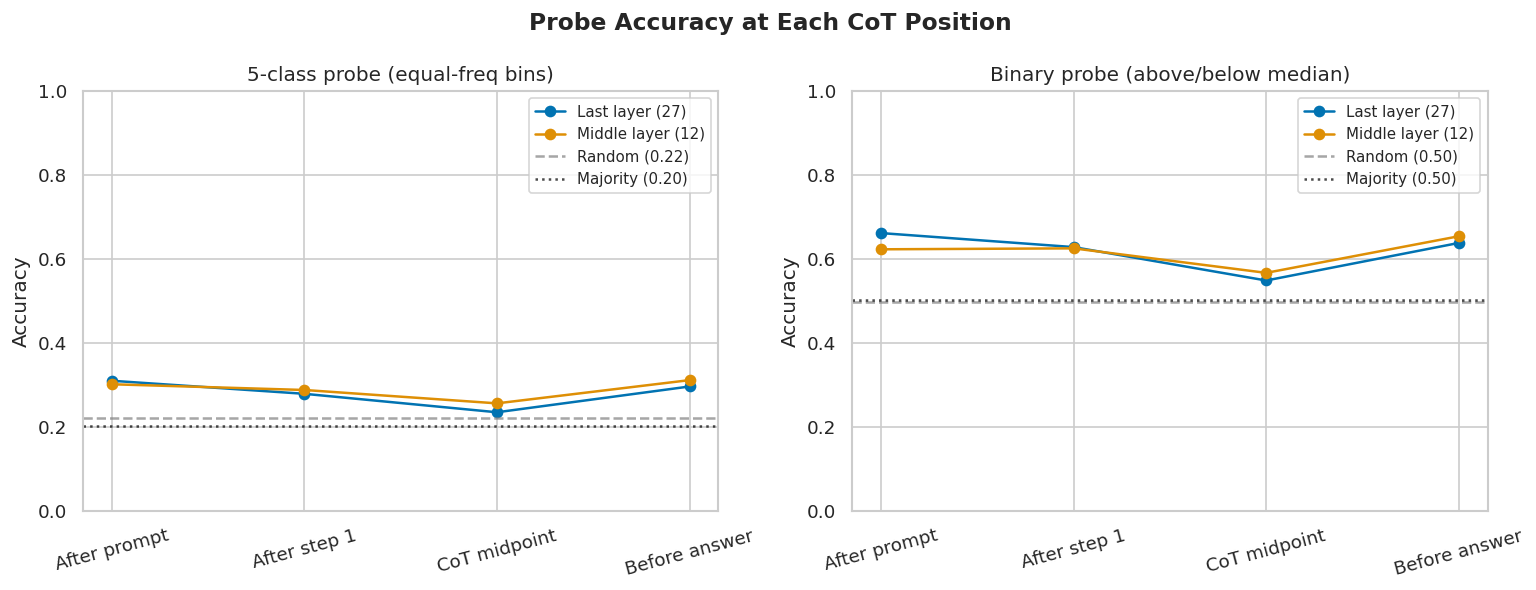
\includegraphics[width=\columnwidth]{../results/figures/probe_accuracy_curve.png}
\caption{Probe accuracy at four CoT positions for last-layer (27) and middle-layer (12) hidden states. Dashed lines show random and majority baselines.}
\label{fig:probe}
\end{figure}

\subsection{Step Corruption}

Of 200 test examples, 47 (23.5\%) contained detectable arithmetic equations suitable for corruption; the remaining examples used prose-style reasoning without explicit equations. Results for the 47 corrupted examples are shown in Table~\ref{tab:corruption} and Figure~\ref{fig:corruption}.

\begin{table}[t]
\centering
\small
\begin{tabular}{lc}
\toprule
\textbf{Metric} & \textbf{Value} \\
\midrule
Examples with equations & 47 / 200 (23.5\%) \\
Answer change rate & 0.149 \\
Error propagation rate & 0.149 \\
Answer unchanged & 0.851 \\
\midrule
Change rate (high drift) & 0.125 \\
Change rate (low drift)  & 0.174 \\
\bottomrule
\end{tabular}
\caption{Step corruption results. High/low drift groups are split at the median hidden-state drift (L2 distance pos0→pos3, layer 27).}
\label{tab:corruption}
\end{table}

The model's final answer changed in only 14.9\% of corruption cases. When the answer did change, the new answer always reflected the corrupted value (error propagation rate = answer change rate = 0.149), meaning the model did not spontaneously correct the error—it simply continued without noticing in 85.1\% of cases.

\subsection{Cross-Check}

Splitting examples by hidden-state drift (low drift = model representation changes little from pos0 to pos3), low-drift examples show a slightly \textit{higher} corruption sensitivity (17.4\%) than high-drift examples (12.5\%). This is a small and likely noisy difference with only 47 examples, and we discuss its interpretation in Section~\ref{sec:analysis}.

\begin{figure}[t]
\centering
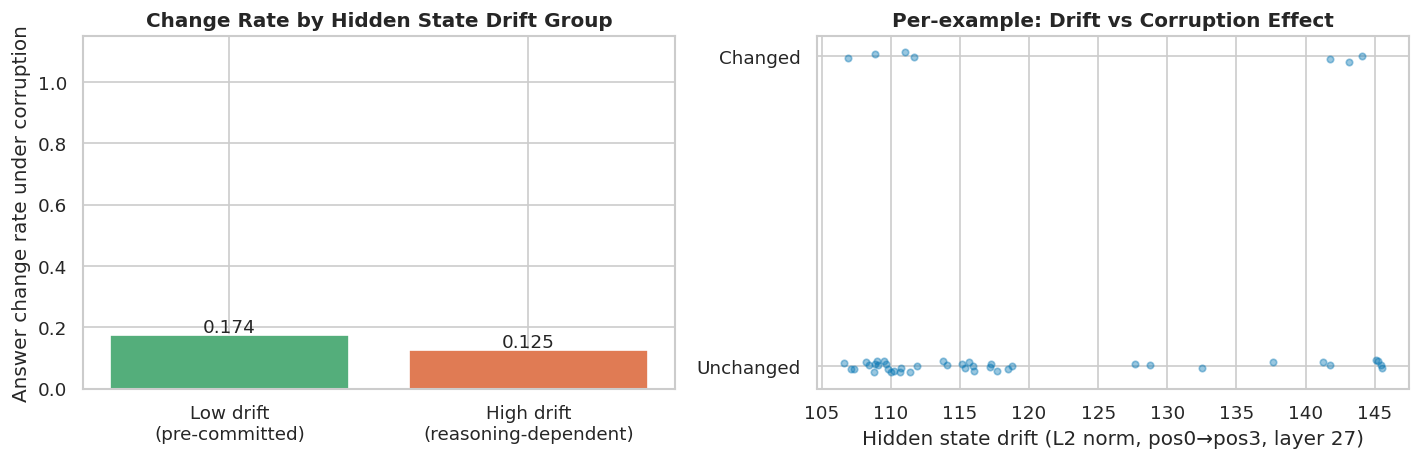
\includegraphics[width=\columnwidth]{../results/figures/crosscheck.png}
\caption{Cross-check results. Left: answer change rate by hidden-state drift group. Right: per-example scatter of drift vs.\ corruption effect.}
\label{fig:corruption}
\end{figure}

\section{Analysis and Discussion}
\label{sec:analysis}

\paragraph{The model encodes answer information early.}
The most striking finding is that binary probe accuracy at pos0—before a single reasoning token is written—is 0.661, far above the 0.202 majority baseline. This means a linear classifier can predict whether the final answer is above or below the median using only the hidden state at the end of the problem prompt. The model has already committed to an answer range before writing any reasoning.

\paragraph{CoT accuracy does not increase across steps.}
Under faithful CoT, we would expect probe accuracy to be low at pos0 and rise as the model works through the problem. Instead, we observe that accuracy is \textit{highest} at pos0, dips at pos2, and partially recovers at pos3. One interpretation is that the reasoning steps introduce noise into the representation—the model is not building toward a new conclusion but elaborating on one already made. The partial recovery at pos3 is consistent with the model re-anchoring to its final answer just before generating it.

\paragraph{Corruption has minimal effect.}
An 85.1\% answer-unchanged rate under step corruption provides further evidence that the model does not genuinely use its written intermediate steps. When we replace \texttt{16 - 3 = **13**} with a wrong value, the model almost always produces the same final answer anyway. This is consistent with the probe finding: if the answer is already encoded early, corrupting a later step cannot change it.

\paragraph{Cross-check interpretation.}
The cross-check result is slightly counterintuitive: low-drift examples (where the hidden state changes little from pos0 to pos3, suggesting the model was "pre-committed" early) showed slightly \textit{higher} corruption sensitivity than high-drift examples. However, the difference is small (17.4\% vs.\ 12.5\%) with only 47 examples in the corrupted subset, so we cannot draw strong conclusions. The overall pattern is consistent with post-hoc rationalization—both groups show low corruption sensitivity in absolute terms.

\paragraph{Limitations.}
\textit{Equation coverage.} Only 47 of 200 examples had detectable equations in the structured solution section of the output. DeepSeek-R1-1.5B writes most of its reasoning in prose inside \texttt{<think>} tags, with explicit equations appearing in a post-think structured summary. Future work should develop corruption methods suited to prose-style reasoning (e.g., corrupting intermediate numbers mentioned in text).

\textit{Binned probe targets.} We predict binned answer categories rather than exact values, which limits interpretability. A probe that perfectly predicts the bin provides weaker evidence than one that predicts the exact answer.

\textit{Model scale.} Our findings are specific to a 1.5B-parameter distilled model. Larger models or models trained differently may exhibit more faithful CoT behavior.

\textit{Probe capacity.} A logistic regression probe can only detect linearly separable information. The model may encode answer information in a nonlinear way that our probes miss at early positions, potentially underestimating early encoding.

\paragraph{Summary.}
Both experiments point in the same direction: the written chain of thought in \textsc{DeepSeek-R1-Distill-Qwen-1.5B} is largely a post-hoc narrative. The model encodes answer information before reasoning begins, and corrupting intermediate steps has little effect on the final answer. This does not mean CoT is useless—it may still improve accuracy by regularizing generation—but it does mean that the written steps cannot be read as a transparent window into the model's computation.

\section*{Acknowledgments}
Compute was provided by Purdue's Rosen Center for Advanced Computing (RCAC) Gilbreth cluster and Lambda GPU Cloud.

\bibliography{references}

\appendix
\section{Implementation Details}
\label{appendix:impl}

All code is available at \url{https://github.com/SameerMurthy5/cot-hidden-state-probing}. The pipeline consists of four scripts run in sequence:

\begin{enumerate}
    \item \texttt{src/generate\_cot.py}: Runs the model on GSM8K, generates CoT traces with greedy decoding, and extracts hidden states at four positions per example using forward passes on prefixes. Outputs \texttt{.jsonl} files with one record per example including the full generated text and hidden state vectors.
    \item \texttt{src/probe.py}: Loads hidden state files, bins ground-truth answers into 5 equal-frequency bins, and trains logistic regression probes (scikit-learn, \texttt{C=1.0}, \texttt{max\_iter=1000}) at each position and layer with an 80/20 train/test split.
    \item \texttt{src/corrupt.py}: Samples 200 test examples, identifies arithmetic equations via regex, corrupts one result per example, re-runs inference, and computes answer change and error propagation rates.
    \item \texttt{src/analyze.py}: Loads \texttt{probe\_results.json} and \texttt{corruption\_results.json} and generates all figures.
\end{enumerate}

Total compute: approximately 15 GPU hours on NVIDIA A10/A30 GPUs.

\end{document}
